\documentclass[dvipsnames, aspectratio=169]{beamer}
\usepackage[utf8]{inputenc}
\usepackage[T1]{fontenc}
\usepackage{tikz}
\usetikzlibrary{shapes.geometric}
\usepackage{standalone}
\usepackage{amsmath}
\usepackage{amsfonts}
\usepackage{graphicx, color}
\usepackage{svg}
\usepackage[]{xcolor}
\usepackage{standalone}
% \usepackage[a4paper,margin=3.5cm]{geometry}
\usepackage{pgfplots}
\pgfplotsset{width=7cm,compat=1.8}
\usepackage{pgfplotstable}
\usepackage{hyperref}


\usepackage[]{biblatex}
\addbibresource{references.bib}

\newcommand{\bA}{\mathbf{A}}
\newcommand{\bB}{\mathbf{B}}
\newcommand{\bb}{\mathbf{b}}
\newcommand{\E}{\mathbb{E}}
\newcommand{\eye}{\mathbb{I}}
\newcommand{\Norm}{\mathcal{N}}
\newcommand{\Loss}{\mathcal{L}}
\newcommand{\py}{\mathbf{p}_y}
\newcommand{\bQ}{\mathbf{Q}}
\newcommand{\R}{\mathbb{R}}
\newcommand{\bR}{\mathbf{R}}
\newcommand{\bt}{\mathbf{t}}
\newcommand{\bU}{\mathbb{U}}
\newcommand{\bu}{\mathbf{u}}
\newcommand{\bw}{\mathbf{w}}
\newcommand{\bX}{\mathbf{X}}
\newcommand{\bx}{\mathbf{x}}
\newcommand{\by}{\mathbf{y}}
\newcommand{\bZ}{\mathbf{Z}}
\newcommand{\bz}{\mathbf{z}}

\newcommand{\eq}{=}
\newcommand{\parfrac}[2]{\frac{\partial #1}{\partial#2}}

\title{Causal Effect Inference with Normalising Flows}
\author{Micha de Groot}


\begin{document}
	
	\begin{frame}
		\titlepage
	\end{frame}
	
	\begin{frame}{Overview of the presentation}
	    \begin{itemize}
	        \item Introduction
	    \end{itemize}
	\end{frame}
	\begin{frame}{Overview of the presentation}
	    \begin{itemize}
	        \item Introduction
	        \item Background on causal inference
	    \end{itemize}
	\end{frame}
	\begin{frame}{Overview of the presentation}
	    \begin{itemize}
	        \item Introduction
	        \item Background on causal inference
	        \item Model we used
	    \end{itemize}
	\end{frame}
	\begin{frame}{Overview of the presentation}
	    \begin{itemize}
	        \item Introduction
	        \item Background on causal inference
	        \item Model we used
	        \item Existing and new datasets
	    \end{itemize}
	\end{frame}
	\begin{frame}{Overview of the presentation}
	    \begin{itemize}
	        \item Introduction
	        \item Background on causal inference
	        \item Model we used
	        \item Existing and new datasets
	        \item Results
	    \end{itemize}
	\end{frame}
		\begin{frame}{Overview of the presentation}
	    \begin{itemize}
	        \item Introduction
	        \item Background on causal inference
	        \item Model we used
	        \item Existing and new datasets
	        \item Results
	        \item Conclusion
	    \end{itemize}
	\end{frame}
	
	\begin{frame}{Introduction}
	    Causal inference is concerned with uncovering causal relationships instead of correlations between observations. This requires explicit modelling of latent confounders.
	    \begin{figure}
	        \centering
	        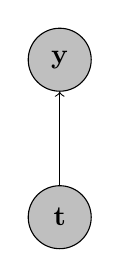
\begin{tikzpicture}
            \node[circle, draw=black, fill=lightgray, minimum size=0.8cm] (t) at (0, 0) {$\mathbf{t}$};
            \node[circle, draw=black, fill=lightgray, minimum size=0.8cm] (y) at (0, 2) {$\mathbf{y}$};

            \draw[->] (t) -- (y);
            \end{tikzpicture}
	        \qquad\qquad
	        \includestandalone{Figures/causal_graph_observed_confounder_no_proxy}
	    \end{figure}
	\end{frame}
	
	\begin{frame}{Introduction}
	    Deep learning, and especially generative modelling is of interest here. Earlier work has attempted this with the Causal VAE (CEVAE).
	\end{frame}
	\begin{frame}{Introduction}
	    Deep learning, and especially generative modelling is of interest here. Earlier work has attempted this with the Causal VAE (CEVAE). But the CEVAE is limited in how well it can model the posterior of the latent confounder.
	    
	    \vspace{0.5cm}
	    Therefore we introduce a Normalising Flow-based model, which allows us to model the posterior over the latent confounder more accurately.
	\end{frame}
	
	\begin{frame}{Introduction}
	    Existing dataset for causal inference are small and simple. Model performance is limited for more complex models.
	\end{frame}
	\begin{frame}{Introduction}
	    Existing dataset for causal inference are small and simple. Model performance is limited for more complex models.
	    
	    Therefore we introduce a new dataset, called Space Shapes, that is higher dimensional and more complex.
	\end{frame}
	
	\begin{frame}{Research questions}
    \begin{enumerate}
        \item Is the accuracy of the posterior approximation relevant for causal modelling? Namely, if we were to rely on Normalising Flow-based models that can learn the true posterior, would that yield a better causal modelling? 
    \end{enumerate} 
	\end{frame}
		\begin{frame}{Research questions}
    \begin{enumerate}
        \item Is the accuracy of the posterior approximation relevant for causal modelling? Namely, if we were to rely on Normalising Flow-based models that can learn the true posterior, would that yield a better causal modelling? 
        \item Does the higher complexity and dimensionality of the new Space Shapes dataset show the improvements of more complex causal inference models?
    \end{enumerate} 
	\end{frame}
	
	\begin{frame}{Background: causal graphs}
	    \begin{figure}
	        \centering
	        \includestandalone{Figures/causal_graph_observed_confounder_no_proxy}
	        \qquad
	        \includestandalone{Figures/causal_graph_independent_intervention_no_proxy}
	        \caption{Causal graph with two observed variables, $\by$ and $\bt$, and their latent confouder $\bz$. On the left hand side before intervening on $\bt$ and on the right hand side after intervening on $\bt$}
	       % \label{fig:my_label}
	    \end{figure}
	\end{frame}
	\begin{frame}{Background: causal graphs}
	    \begin{figure}
	        \centering
	        \includestandalone{Figures/causal_graph_one_proxy_one_confounder}
	        \qquad
	        \includestandalone{Figures/causal_graph_independent_intervention}
	        \caption{Causal graph with a proxy variable $\bx$. On the left hand side before intervening on $\bt$ and on the right hand side after intervening on $\bt$}
	       % \label{fig:my_label}
	    \end{figure}
	\end{frame}
	\begin{frame}{Background: formalisation of an intervention with \textit{do}-calculus}
	    We formalise the notion of an intervention by introducing the \textit{do}-operator in probability theory.
	    
	    \noindent
	    Classical likelihood estimation:
	    \begin{equation}\color{Blue}p(\by|\bt) \color{black}= \int_\bz \color{ForestGreen}p(\by|\bt, \bz) \color{orange}p(\bz|\bt) \color{black}d\bz \end{equation}
	    \vspace{1cm}
	    Causal inference estimation:
	    \begin{equation}\begin{split}
	        \color{Blue}p(\by|do(\bt)) &= \int_\bz \color{ForestGreen}p(\by|do(\bt), \bz) \color{orange}p(\bz|do(\bt)) \color{black}d\bz\\
	        &= \int_\bz \color{ForestGreen}p(\by|\bt, \bz) \color{orange}p(\bz) \color{black}d\bz
	    \end{split}\end{equation}
	\end{frame}
	\begin{frame}{Background: formalisation of an intervention with \textit{do}-calculus}
	    Adding our proxy variable gives the following equation:
	    \begin{equation}\label{equation:prediction_of_do_t}
        \begin{split}
            \color{Blue}p(\by | \bx, do(\bt)) &= \int_{\bz} \color{ForestGreen}p(\by | \bx, do(\bt), \bz) \color{orange}p(\bz | \bx, do(\bt)) \color{black}d\bz\\
            &= \int_{\bz} \color{ForestGreen}p(\by|\bt, \bz) \color{orange}p(\bz|\bx) \color{black}d\bz
        \end{split}
        \end{equation}
	\end{frame}
	\begin{frame}{Background: metrics}
	    It is common to look at a binary difference between two interventions. At the Average Treatment Effect (ATE)
	    \begin{equation}
	        ATE := \E[\color{Blue}\by|do(\bt=1)\color{black}] - \E[\color{Blue}\by |do(\bt=0)\color{black}]
	    \end{equation}
	    
	    \vspace{0.5cm}
	    And secondly at the Individual Treatment Effect (ITE):
	    \begin{equation}
	        ITE(x) := \E[\color{Blue}\by|\bx=x, do(\bt=1)\color{black}] - \E[\color{Blue}\by | \bx=x, do(\bt=0)\color{black}]
	    \end{equation}
	\end{frame}
	\begin{frame}{Background: metrics}
	    For the ATE we use the absolute error of the ATE as a measure of accuracy:
	    \begin{equation}
	        ATE_{err} := \left|ATE - ATE_{estim} \right|
	    \end{equation}
	    
	    \vspace{0.5cm}
	    And for the ITE the root mean squared error:
	    \begin{equation}
	        ITE_{err} := \sqrt{\frac{1}{N} \sum\limits^N_{i=1} (ITE(x_i) - ITE_{estim}(x_i))^2}
	    \end{equation}
	\end{frame}
	\begin{frame}{Background: metrics}
	    The third metric is the Precision in Estimation of Heterogeneous Effect (PEHE):
	    \begin{equation}
	        PEHE := \frac{1}{N}\sum\limits^N_{i=1}((\by_{i1} - \by_{i0}) - (\hat{\by}_{i1} - \hat{\by}_{i0}))^2    
	    \end{equation}
	    With $\by$ and $\hat{\by}$ the real outcome value for a certain intervention value and the predicted outcome for a certain intervention value respectively.
	\end{frame}
	
	\begin{frame}{Models}
	    \begin{figure}
            \centering
            \includestandalone[width=0.53\textwidth]{Figures/cevae_encoder_figure}
            \includestandalone[width=0.39\textwidth]{Figures/cevae_decoder_figure}
            \caption{Graph of the encoder and decoder of the CEVAE. Nodes in white are feed forward neural networks and nodes in grey are sampling steps or data input.}
        \end{figure}
	\end{frame}
	\begin{frame}{Models}
    	 We use Normalising Flows in two ways. 
    	 \begin{itemize}
    	     \item Extending the CEVAE with a Normalising Flow posterior
    	     \item Introduce a new Flow-based model
    	 \end{itemize}
	\end{frame}
	
	\begin{frame}{Models: what are Normalising Flows}
	    Learn an invertible mapping $f$ between data and latent variable:
	    \begin{equation}\label{equation:change_of_variables}
        {\color{ForestGreen}\bx} = {\color{Blue}f(\bz)} \qquad {\color{ForestGreen}p(\bx)} = {\color{Blue}p(\bz)} \left|\text{det} \parfrac{{\color{Blue}f}}{\color{Blue}\bz} \right|^{-1}
        \end{equation}

        In practice we optimise the log and split $f$ into a series of such transformations.
	    \begin{equation}\label{equation:change_of_variables_log_chain}
        \ln{\color{ForestGreen} p(\bx)} = \ln {\color{Blue}p(\bz_0)} - \sum\limits^K_{k=1}\ln \left| \text{det} \parfrac{\color{Blue}f_k}{\color{Blue}\bz_{k-1}} \right|
        \end{equation}
	\end{frame}

    \begin{frame}{Models: How do we use Normalising Flows}
        Extend CEVAE:
        \begin{figure}
            \centering
            \includestandalone{Figures/cenf_with_vae}
            \caption{Visualisation of the CEVAE, augmented with a normalising flow. The encoder part on the left and the decoder part on the right is the same as before.}
            % \label{fig:cenf_with_vae}
        \end{figure}
        We test this with three types of flow functions
    \end{frame}
    
    \begin{frame}{Models: How do we use Normalising Flows}
        Make connections in the graph a Normalising Flow.
        \begin{figure}
            \centering
            \includestandalone{Figures/causal_graph_one_proxy_one_confounder}
            \hspace{2cm}
            \includestandalone{Figures/causal_graph_prior_at_outcome}
            \caption{The causal graph in the original formulation on the right hand side and the causal graph with an added prior on the left hand side.}
            \label{fig:graph_prior_at_outcome}
        \end{figure}
    \end{frame}
    
    \begin{frame}{Models: How do we use Normalising Flows}
        We add a new variable and learn two Normalising Flows: $\color{Blue}f$ and $\color{DarkOrchid}g$
        \begin{equation}
            {\color{ForestGreen}\bx} = {\color{Blue}f_K \circ ... \circ f_1(\bz_0)}, \qquad \ln {\color{ForestGreen}p(\bx)} = \ln {\color{Blue}p(\bz_0)} - \sum\limits^K_{k=1} \ln \left|\det \parfrac{\color{Blue}f_k}{\color{Blue}\bz_{k-1}}\right| 
        \end{equation}
        \begin{equation}
            {\color{RedOrange}\by_K} = {\color{DarkOrchid}g_K \circ ... \circ g_1(\py;} {\color{Blue}\bt, \bz}{\color{DarkOrchid})}, \quad \ln {\color{RedOrange}p(\by_K)} = \ln {\color{DarkOrchid}p(\py)} - \sum\limits^K_{k=1} \ln \left|\det \parfrac{\color{DarkOrchid}g_k}{\color{DarkOrchid}\by_{k-1}}\right| 
        \end{equation}
        We test this with two types of flow functions. 
    \end{frame}
    \begin{frame}
        \begin{figure}[h]
            \centering
            \includestandalone[width=0.45\textwidth]{Figures/causal_flow_with_y_prior_training}
            \qquad
            \includestandalone[width=0.45\textwidth]{Figures/causal_flow_with_y_prior_testing}
            \caption{Causal Inference Flow model. The graph on the left hand side indicates the direction of the flows during training and the graph on the right hand side indicates the direction of the flow during testing. }
        \end{figure}
    \end{frame}
	
	\begin{frame}{Existing datasets}
	    \begin{itemize}
	        \item Infant Healt and Development Program (IHDP)
	        \item Twin birth research (TWINS)
	    \end{itemize}
	\end{frame}
	\begin{frame}{New dataset: Space Shapes}
	    \begin{figure}
	        \centering
	        \includegraphics[width=1.0\textwidth]{latex/Images/sample_space_shapes_score_left.png}
	        \caption{Sample of the Space Shapes dataset. Observed variables on the right. The image on the right is a visualisation of the process that underlies the outcome variable, but is never observed. The movement vector is the combined effect of the intervention variable and the 'Gravity' effects.}
	    \end{figure}
	\end{frame}
	\begin{frame}{New dataset: post-training modifications}
	    We selected three modifications to apply to the data after the models were trained:
	    \begin{itemize}
	        \item Have fewer objects in the image
	        \item Swap objects with objects that have a different shape/colour combination
	        \item Change the size of the objects in the image randomly
	    \end{itemize}
	\end{frame}

	
	\begin{frame}{Results: Average Treatment Effect}
	    \begin{figure}[h]
	    \hspace{3cm}
        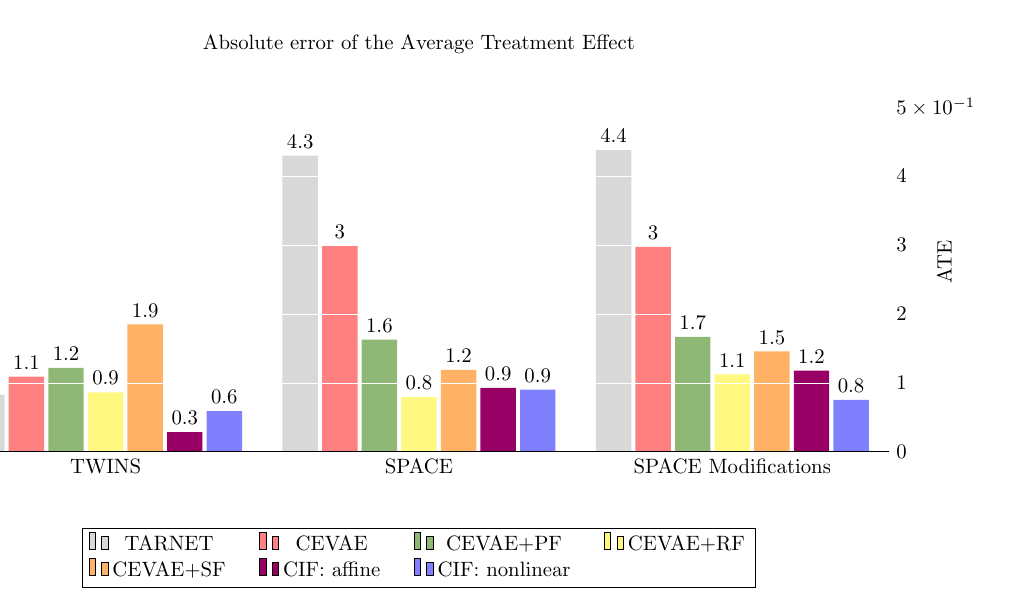
\begin{tikzpicture}[trim left=1cm, scale=0.75]
            \begin{axis}[
                ybar, axis on top,
                title={Absolute error of the Average Treatment Effect},
                height=8cm, width=17.5cm,
                bar width=0.6cm,
                % bar shift=-0.3,
                xtick=data,
                ymajorgrids, tick align=inside,
                major grid style={draw=white},
                enlarge x limits=0.25,
                enlarge y limits={value=.1,upper},
                ymin=0, ymax=5,
                ytick={0, 1, 2, 3, 4, 5},
                yticklabels={0, 1, 2, 3, 4, $5\times10^{-1}$},
                axis x line*=bottom,
                axis y line*=right,
                y axis line style={opacity=0},
                tickwidth=0pt,
                % enlarge x limits=true,
                legend style={
                    at={(0.5,-0.2)},
                    anchor=north,
                    legend columns=4,
                    /tikz/every even column/.append style={column sep=0.5cm}
                },
                ylabel shift=-25pt,
                ylabel={ATE},
                symbolic x coords={
                   TWINS, SPACE, SPACE Modifications},
                nodes near coords={
                \pgfmathprintnumber[precision=1, fixed]{\pgfplotspointmeta}
               }
            ]
            \addplot [draw=none, fill=gray!30] coordinates {
              (TWINS, 0.83) 
              (SPACE, 4.30)
              (SPACE Modifications, 4.38)};
            \addplot [draw=none,fill=red!50] coordinates {
              (TWINS, 1.09) 
              (SPACE, 2.99)
              (SPACE Modifications, 2.975)};
            \addplot [draw=none, fill=OliveGreen!50] coordinates {
              (TWINS, 1.22) 
              (SPACE, 1.63)
              (SPACE Modifications, 1.67)};
            \addplot [draw=none, fill=yellow!50] coordinates {
              (TWINS, 0.864) 
              (SPACE, 0.796)
              (SPACE Modifications, 1.124)};
            \addplot [draw=none, fill=orange!60] coordinates {
              (TWINS, 1.85) 
              (SPACE, 1.189)
              (SPACE Modifications, 1.458)};
            \addplot [draw=none, fill=red!60!blue] coordinates {
              (TWINS, 0.285) 
              (SPACE, 0.930)
              (SPACE Modifications, 1.18)};
            \addplot [draw=none, fill=blue!50] coordinates {
              (TWINS, 0.591) 
              (SPACE, 0.904)
              (SPACE Modifications, 0.756)};
            \legend{TARNET, CEVAE, CEVAE+PF, CEVAE+RF, CEVAE+SF, CIF: affine, CIF: nonlinear}
            % \node[draw=black, fill=white] (a) at (13,730) {$6+$};
            \end{axis}
        \end{tikzpicture}
        % \caption{Average Treatment effect scores for all models.  The SPACE Modifications data is the average over all three distributional shifts of the Space Shapes dataset. The standard deviation for all models was approximately $10^{-2}$}
        \label{fig:ATE}
        \end{figure}
	\end{frame}
    \begin{frame}{Results: Average Treatment Effect}
	    \begin{figure}[h]
	    \hspace{3cm}
        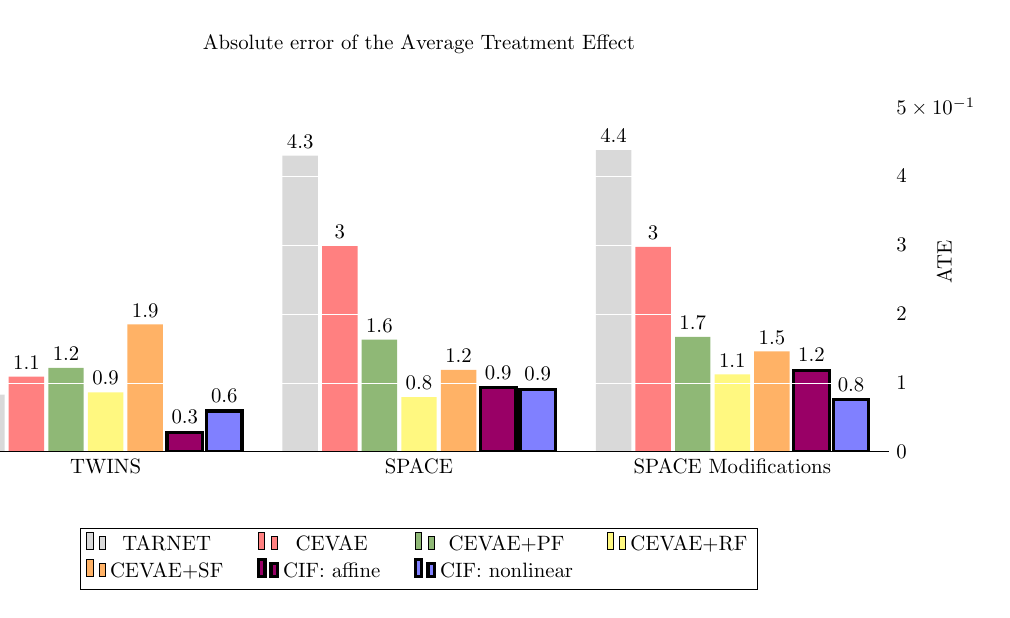
\begin{tikzpicture}[trim left=1cm, scale=0.75]
            \begin{axis}[
                ybar, axis on top,
                title={Absolute error of the Average Treatment Effect},
                height=8cm, width=17.5cm,
                bar width=0.6cm,
                % bar shift=-0.3,
                xtick=data,
                ymajorgrids, tick align=inside,
                major grid style={draw=white},
                enlarge x limits=0.25,
                enlarge y limits={value=.1,upper},
                ymin=0, ymax=5,
                ytick={0, 1, 2, 3, 4, 5},
                yticklabels={0, 1, 2, 3, 4, $5\times10^{-1}$},
                axis x line*=bottom,
                axis y line*=right,
                y axis line style={opacity=0},
                tickwidth=0pt,
                % enlarge x limits=true,
                legend style={
                    at={(0.5,-0.2)},
                    anchor=north,
                    legend columns=4,
                    /tikz/every even column/.append style={column sep=0.5cm}
                },
                ylabel shift=-25pt,
                ylabel={ATE},
                symbolic x coords={
                   TWINS, SPACE, SPACE Modifications},
                nodes near coords={
                \pgfmathprintnumber[precision=1, fixed]{\pgfplotspointmeta}
               }
            ]
            \addplot [draw=none, fill=gray!30] coordinates {
              (TWINS, 0.83) 
              (SPACE, 4.30)
              (SPACE Modifications, 4.38)};
            \addplot [draw=none,fill=red!50] coordinates {
              (TWINS, 1.09) 
              (SPACE, 2.99)
              (SPACE Modifications, 2.975)};
            \addplot [draw=none, fill=OliveGreen!50] coordinates {
              (TWINS, 1.22) 
              (SPACE, 1.63)
              (SPACE Modifications, 1.67)};
            \addplot [draw=none, fill=yellow!50] coordinates {
              (TWINS, 0.864) 
              (SPACE, 0.796)
              (SPACE Modifications, 1.124)};
            \addplot [draw=none, fill=orange!60] coordinates {
              (TWINS, 1.85) 
              (SPACE, 1.189)
              (SPACE Modifications, 1.458)};
            \addplot [draw=black, ultra thick, fill=red!60!blue] coordinates {
              (TWINS, 0.285) 
              (SPACE, 0.930)
              (SPACE Modifications, 1.18)};
            \addplot [draw=black, ultra thick, fill=blue!50] coordinates {
              (TWINS, 0.591) 
              (SPACE, 0.904)
              (SPACE Modifications, 0.756)};
            \legend{TARNET, CEVAE, CEVAE+PF, CEVAE+RF, CEVAE+SF, CIF: affine, CIF: nonlinear}
            % \node[draw=black, fill=white] (a) at (13,730) {$6+$};
            \end{axis}
        \end{tikzpicture}
        % \caption{Average Treatment effect scores for all models.  The SPACE Modifications data is the average over all three distributional shifts of the Space Shapes dataset. The standard deviation for all models was approximately $10^{-2}$}
        \label{fig:ATE}
        \end{figure}
	\end{frame}	
	\begin{frame}{Results: Average Treatment Effect}
	    \begin{figure}[h]
	    \hspace{3cm}
        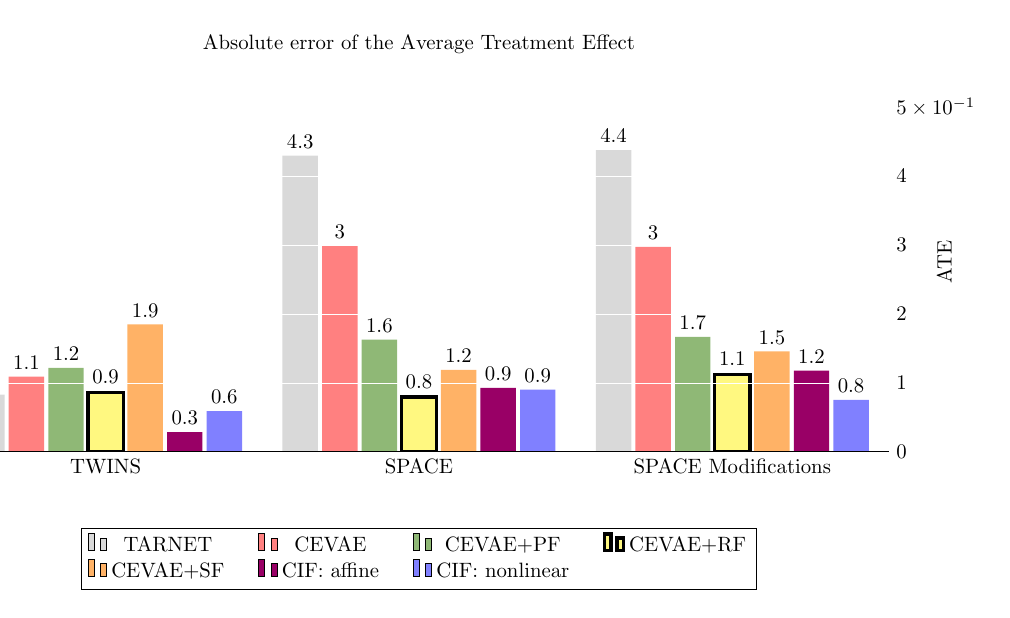
\begin{tikzpicture}[trim left=1cm, scale=0.75]
            \begin{axis}[
                ybar, axis on top,
                title={Absolute error of the Average Treatment Effect},
                height=8cm, width=17.5cm,
                bar width=0.6cm,
                % bar shift=-0.3,
                xtick=data,
                ymajorgrids, tick align=inside,
                major grid style={draw=white},
                enlarge x limits=0.25,
                enlarge y limits={value=.1,upper},
                ymin=0, ymax=5,
                ytick={0, 1, 2, 3, 4, 5},
                yticklabels={0, 1, 2, 3, 4, $5\times10^{-1}$},
                axis x line*=bottom,
                axis y line*=right,
                y axis line style={opacity=0},
                tickwidth=0pt,
                % enlarge x limits=true,
                legend style={
                    at={(0.5,-0.2)},
                    anchor=north,
                    legend columns=4,
                    /tikz/every even column/.append style={column sep=0.5cm}
                },
                ylabel shift=-25pt,
                ylabel={ATE},
                symbolic x coords={
                   TWINS, SPACE, SPACE Modifications},
                nodes near coords={
                \pgfmathprintnumber[precision=1, fixed]{\pgfplotspointmeta}
               }
            ]
            \addplot [draw=none, fill=gray!30] coordinates {
              (TWINS, 0.83) 
              (SPACE, 4.30)
              (SPACE Modifications, 4.38)};
            \addplot [draw=none,fill=red!50] coordinates {
              (TWINS, 1.09) 
              (SPACE, 2.99)
              (SPACE Modifications, 2.975)};
            \addplot [draw=none, fill=OliveGreen!50] coordinates {
              (TWINS, 1.22) 
              (SPACE, 1.63)
              (SPACE Modifications, 1.67)};
            \addplot [draw=black, ultra thick, fill=yellow!50] coordinates {
              (TWINS, 0.864) 
              (SPACE, 0.796)
              (SPACE Modifications, 1.124)};
            \addplot [draw=none, fill=orange!60] coordinates {
              (TWINS, 1.85) 
              (SPACE, 1.189)
              (SPACE Modifications, 1.458)};
            \addplot [draw=none, fill=red!60!blue] coordinates {
              (TWINS, 0.285) 
              (SPACE, 0.930)
              (SPACE Modifications, 1.18)};
            \addplot [draw=none, fill=blue!50] coordinates {
              (TWINS, 0.591) 
              (SPACE, 0.904)
              (SPACE Modifications, 0.756)};
            \legend{TARNET, CEVAE, CEVAE+PF, CEVAE+RF, CEVAE+SF, CIF: affine, CIF: nonlinear}
            % \node[draw=black, fill=white] (a) at (13,730) {$6+$};
            \end{axis}
        \end{tikzpicture}
        % \caption{Average Treatment effect scores for all models.  The SPACE Modifications data is the average over all three distributional shifts of the Space Shapes dataset. The standard deviation for all models was approximately $10^{-2}$}
        \label{fig:ATE}
        \end{figure}
	\end{frame}	
	
	
	
	
	
	
	\begin{frame}{Results: Individual Treatment Effect}
	    \begin{figure}[h]
	    \hspace{3cm}
        % \begin{tikzpicture}[trim left=1cm, scale=0.6]
        \begin{tikzpicture}[trim left=1cm, scale=0.75]
                \begin{axis}[
                    ybar, axis on top,
                    title={Root mean squared error of Individual Treatment Effect},
                    height=8cm, width=17.5cm,
                    bar width=0.6cm,
                    % bar shift=-0.3,
                    xtick=data,
                    ymajorgrids, tick align=inside,
                    major grid style={draw=white},
                    enlarge x limits=0.25,
                    enlarge y limits={value=.1,upper},
                    ymin=0, ymax=3,
                    ytick={0, 0.5, 1, 1.5, 2, 2.5, 3},
                    % yticklabels={0, 1, 2, 3, 4, 5, $6$},
                    axis x line*=bottom,
                    axis y line*=right,
                    y axis line style={opacity=0},
                    tickwidth=0pt,
                    % enlarge x limits=true,
                    legend style={
                        at={(0.5,-0.2)},
                        anchor=north,
                        legend columns=4,
                        /tikz/every even column/.append style={column sep=0.5cm}
                    },
                    ylabel={ITE},
                    symbolic x coords={
                       TWINS, SPACE, SPACE Modifications},
                   nodes near coords={
                    \pgfmathprintnumber[precision=1, fixed]{\pgfplotspointmeta}
                   }
                ]
                \addplot [draw=none, fill=gray!30] coordinates {
                  (TWINS, 0.65) 
                  (SPACE, 2.19)
                  (SPACE Modifications, 2.37)};
                \addplot [draw=none,fill=red!50] coordinates {
                  (TWINS, 0.384) 
                  (SPACE, 1.637)
                  (SPACE Modifications, 1.78)};
                \addplot [draw=none, fill=OliveGreen!50] coordinates {
                  (TWINS, 0.383) 
                  (SPACE, 1.601)
                  (SPACE Modifications, 1.769)};
                \addplot [draw=none, fill=yellow!50] coordinates {
                  (TWINS, 0.938) 
                  (SPACE, 1.890)
                  (SPACE Modifications, 2.104)};
                \addplot [draw=none, fill=orange!60] coordinates {
                  (TWINS, 0.94) 
                  (SPACE, 1.890)
                  (SPACE Modifications, 1.95)};
                \addplot [draw=none, fill=red!60!blue] coordinates {
                  (TWINS, 0.673) 
                  (SPACE, 1.839)
                  (SPACE Modifications, 1.934)};
                \addplot [draw=none, fill=blue!50] coordinates {
                  (TWINS, 0.652) 
                  (SPACE, 1.891)
                  (SPACE Modifications, 2.152)};
                \legend{TARNET, CEVAE, CEVAE+PF, CEVAE+RF, CEVAE+SF, CIF: affine, CIF: nonlinear}
                \end{axis}
            \end{tikzpicture}
            % \caption{Individual Treatment effect scores for all models. The SPACE Modifications data is the average over all three distributional shifts of the Space Shapes dataset. The standard deviation for all models was approximately $10^{-1}$}
            \label{fig:ITE}
        \end{figure}
	\end{frame}
		\begin{frame}{Results: Individual Treatment Effect}
	    \begin{figure}[h]
	    \hspace{3cm}
        % \begin{tikzpicture}[trim left=1cm, scale=0.6]
        \begin{tikzpicture}[trim left=1cm, scale=0.75]
                \begin{axis}[
                    ybar, axis on top,
                    title={Root mean squared error of Individual Treatment Effect},
                    height=8cm, width=17.5cm,
                    bar width=0.6cm,
                    % bar shift=-0.3,
                    xtick=data,
                    ymajorgrids, tick align=inside,
                    major grid style={draw=white},
                    enlarge x limits=0.25,
                    enlarge y limits={value=.1,upper},
                    ymin=0, ymax=3,
                    ytick={0, 0.5, 1, 1.5, 2, 2.5, 3},
                    % yticklabels={0, 1, 2, 3, 4, 5, $6$},
                    axis x line*=bottom,
                    axis y line*=right,
                    y axis line style={opacity=0},
                    tickwidth=0pt,
                    % enlarge x limits=true,
                    legend style={
                        at={(0.5,-0.2)},
                        anchor=north,
                        legend columns=4,
                        /tikz/every even column/.append style={column sep=0.5cm}
                    },
                    ylabel={ITE},
                    symbolic x coords={
                       TWINS, SPACE, SPACE Modifications},
                   nodes near coords={
                    \pgfmathprintnumber[precision=1, fixed]{\pgfplotspointmeta}
                   }
                ]
                \addplot [draw=none, fill=gray!30] coordinates {
                  (TWINS, 0.65) 
                  (SPACE, 2.19)
                  (SPACE Modifications, 2.37)};
                \addplot [draw=black, ultra thick, fill=red!50] coordinates {
                  (TWINS, 0.384) 
                  (SPACE, 1.637)
                  (SPACE Modifications, 1.78)};
                \addplot [draw=black, ultra thick, fill=OliveGreen!50] coordinates {
                  (TWINS, 0.383) 
                  (SPACE, 1.601)
                  (SPACE Modifications, 1.769)};
                \addplot [draw=none, fill=yellow!50] coordinates {
                  (TWINS, 0.938) 
                  (SPACE, 1.890)
                  (SPACE Modifications, 2.104)};
                \addplot [draw=none, fill=orange!60] coordinates {
                  (TWINS, 0.94) 
                  (SPACE, 1.890)
                  (SPACE Modifications, 1.95)};
                \addplot [draw=none, fill=red!60!blue] coordinates {
                  (TWINS, 0.673) 
                  (SPACE, 1.839)
                  (SPACE Modifications, 1.934)};
                \addplot [draw=none, fill=blue!50] coordinates {
                  (TWINS, 0.652) 
                  (SPACE, 1.891)
                  (SPACE Modifications, 2.152)};
                \legend{TARNET, CEVAE, CEVAE+PF, CEVAE+RF, CEVAE+SF, CIF: affine, CIF: nonlinear}
                \end{axis}
            \end{tikzpicture}
            % \caption{Individual Treatment effect scores for all models. The SPACE Modifications data is the average over all three distributional shifts of the Space Shapes dataset. The standard deviation for all models was approximately $10^{-1}$}
            \label{fig:ITE}
        \end{figure}
	\end{frame}
	
	
	
	
	\begin{frame}{Results: Precision in estimation of Heterogeneous Effect}
	    \begin{figure}
	        \hspace{3cm}
            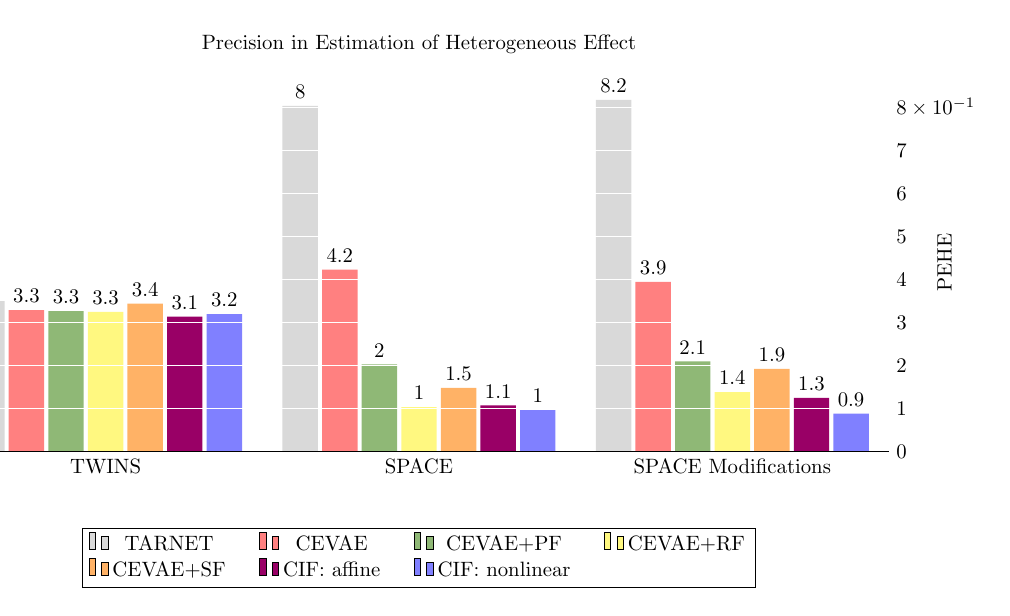
\begin{tikzpicture}[trim left=1cm, scale=0.75]
                % \centering
                \begin{axis}[
                    ybar, axis on top,
                    title={Precision in Estimation of Heterogeneous Effect},
                    height=8cm, width=17.5cm,
                    bar width=0.6cm,
                    % bar shift=-0.3,
                    xtick=data,
                    ymajorgrids, tick align=inside,
                    major grid style={draw=white},
                    enlarge x limits=0.25,
                    enlarge y limits={value=.1,upper},
                    ymin=0, ymax=8,
                    ytick={0, 1, 2, 3, 4, 5, 6, 7, 8},
                    yticklabels={0, 1, 2, 3, 4, 5, 6, 7, $8\times10^{-1}$},
                    axis x line*=bottom,
                    axis y line*=right,
                    y axis line style={opacity=0},
                    tickwidth=0pt,
                    % enlarge x limits=true,
                    legend style={
                        at={(0.5,-0.2)},
                        anchor=north,
                        legend columns=4,
                        /tikz/every even column/.append style={column sep=0.5cm}
                    },
                    ylabel shift=-25pt,
                    ylabel={PEHE},
                    symbolic x coords={
                       TWINS, SPACE, SPACE Modifications},
                   nodes near coords={
                    \pgfmathprintnumber[precision=1, fixed]{\pgfplotspointmeta}
                   }
                ]
                \addplot [draw=none, fill=gray!30] coordinates {
                  (TWINS, 3.50) 
                  (SPACE, 8.03)
                  (SPACE Modifications, 8.17)};
                \addplot [draw=none,fill=red!50] coordinates {
                  (TWINS, 3.29) 
                  (SPACE, 4.23)
                  (SPACE Modifications, 3.944)};
                \addplot [draw=none, fill=OliveGreen!50] coordinates {
                  (TWINS, 3.27) 
                  (SPACE, 2.03)
                  (SPACE Modifications, 2.099)};
                \addplot [draw=none, fill=yellow!50] coordinates {
                  (TWINS, 3.25) 
                  (SPACE, 1.04)
                  (SPACE Modifications, 1.385)};
                \addplot [draw=none, fill=orange!60] coordinates {
                  (TWINS, 3.44) 
                  (SPACE, 1.486)
                  (SPACE Modifications, 1.924)};
                \addplot [draw=none, fill=red!60!blue] coordinates {
                  (TWINS, 3.14) 
                  (SPACE, 1.08)
                  (SPACE Modifications, 1.255)};
                \addplot [draw=none, fill=blue!50] coordinates {
                  (TWINS, 3.20) 
                  (SPACE, 0.971)
                  (SPACE Modifications, 0.887)};
                \legend{TARNET, CEVAE, CEVAE+PF, CEVAE+RF, CEVAE+SF, CIF: affine, CIF: nonlinear}
                \end{axis}
            \end{tikzpicture}
            % \caption{Precision in Estimation of Heterogeneous Effect for all models. The SPACE Modifications data is the average over all three distributional shifts of the Space Shapes dataset. The standard deviation for all models was approximately $10^{-2}$}
            \label{fig:PEHE}
            \end{figure}
	\end{frame}
		\begin{frame}{Results: Precision in estimation of Heterogeneous Effect}
	    \begin{figure}
	        \hspace{3cm}
            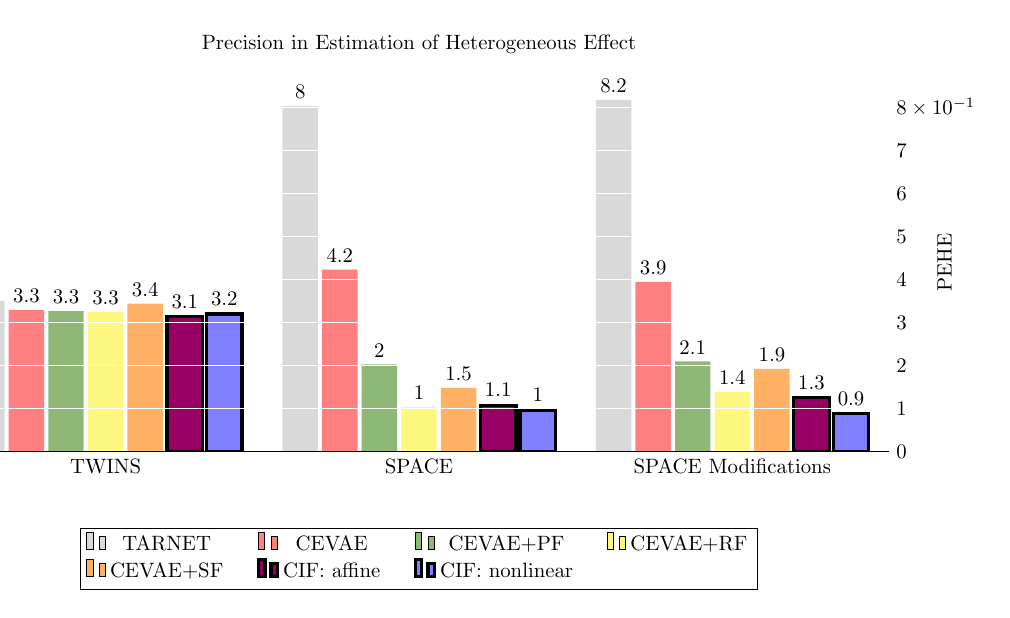
\begin{tikzpicture}[trim left=1cm, scale=0.75]
                % \centering
                \begin{axis}[
                    ybar, axis on top,
                    title={Precision in Estimation of Heterogeneous Effect},
                    height=8cm, width=17.5cm,
                    bar width=0.6cm,
                    % bar shift=-0.3,
                    xtick=data,
                    ymajorgrids, tick align=inside,
                    major grid style={draw=white},
                    enlarge x limits=0.25,
                    enlarge y limits={value=.1,upper},
                    ymin=0, ymax=8,
                    ytick={0, 1, 2, 3, 4, 5, 6, 7, 8},
                    yticklabels={0, 1, 2, 3, 4, 5, 6, 7, $8\times10^{-1}$},
                    axis x line*=bottom,
                    axis y line*=right,
                    y axis line style={opacity=0},
                    tickwidth=0pt,
                    % enlarge x limits=true,
                    legend style={
                        at={(0.5,-0.2)},
                        anchor=north,
                        legend columns=4,
                        /tikz/every even column/.append style={column sep=0.5cm}
                    },
                    ylabel shift=-25pt,
                    ylabel={PEHE},
                    symbolic x coords={
                       TWINS, SPACE, SPACE Modifications},
                   nodes near coords={
                    \pgfmathprintnumber[precision=1, fixed]{\pgfplotspointmeta}
                   }
                ]
                \addplot [draw=none, fill=gray!30] coordinates {
                  (TWINS, 3.50) 
                  (SPACE, 8.03)
                  (SPACE Modifications, 8.17)};
                \addplot [draw=none,fill=red!50] coordinates {
                  (TWINS, 3.29) 
                  (SPACE, 4.23)
                  (SPACE Modifications, 3.944)};
                \addplot [draw=none, fill=OliveGreen!50] coordinates {
                  (TWINS, 3.27) 
                  (SPACE, 2.03)
                  (SPACE Modifications, 2.099)};
                \addplot [draw=none, fill=yellow!50] coordinates {
                  (TWINS, 3.25) 
                  (SPACE, 1.04)
                  (SPACE Modifications, 1.385)};
                \addplot [draw=none, fill=orange!60] coordinates {
                  (TWINS, 3.44) 
                  (SPACE, 1.486)
                  (SPACE Modifications, 1.924)};
                \addplot [draw=black, ultra thick, fill=red!60!blue] coordinates {
                  (TWINS, 3.14) 
                  (SPACE, 1.08)
                  (SPACE Modifications, 1.255)};
                \addplot [draw=black, ultra thick, fill=blue!50] coordinates {
                  (TWINS, 3.20) 
                  (SPACE, 0.971)
                  (SPACE Modifications, 0.887)};
                \legend{TARNET, CEVAE, CEVAE+PF, CEVAE+RF, CEVAE+SF, CIF: affine, CIF: nonlinear}
                \end{axis}
            \end{tikzpicture}
            % \caption{Precision in Estimation of Heterogeneous Effect for all models. The SPACE Modifications data is the average over all three distributional shifts of the Space Shapes dataset. The standard deviation for all models was approximately $10^{-2}$}
            \label{fig:PEHE}
            \end{figure}
	\end{frame}
	
	\begin{frame}{Conclusion}
	    The Causal Inference Flow does quite well at the tasks, though not the best in all scores.
	\end{frame}
	\begin{frame}{Conclusion}
	    The Normalising Flow extensions of the CEVAE does lead to improvement over the CEVAE, but not consistently.
	\end{frame}
	\begin{frame}{Conclusion}
	    The Space Shapes dataset does show a clearer distinction in performance between models.
	    
	    The post-training adaptation on the Space Shape dataset does not dramatically reduce performance of the models
	\end{frame}
	\begin{frame}{Future work}
	    \begin{itemize}
	        \item Test adaptations of the Space Shapes dataset more extensively.
	    \end{itemize}
	\end{frame}
		\begin{frame}{Future work}
	    \begin{itemize}
	        \item Test adaptations of the Space Shapes dataset more extensively.
	        \item Find real-world datasets with similar complexity
	    \end{itemize}
	\end{frame}
	
	
	\begin{frame}{The end}
	    Thank you
	\end{frame}
	
	\begin{frame}{Details on ITE for arbitrary interventions}
	\begin{equation}
        \begin{split}
        ITE(x) &:= \E[\by | \bx=x, do(\bt=1)] - \E[\by | \bx=x, do(\bt=0)]\\
        &:= \E[\by | \bx=x, do(\bt=t_1)] - \E[\by | \bx=x, do(\bt=t_0)],\\
        &\quad t_1 \sim \delta_1, \quad t_0 \sim \delta_0\\
        \end{split}
    \end{equation}
    where $\delta_1$ and $\delta_0$ are Dirac deltas. We can now simply swap out $\delta_1$ and $\delta_0$ with the distributions of interest and then apply the formula. Specifically, we replace them with two normal distributions:
    \begin{equation}
        \begin{split}
        ITE(x) &:= \E[\by | \bx=x, do(\bt=t_1)] - \E[\by | \bx=x, do(\bt=t_0)], \\
        t_1 &\sim \Norm\left(\begin{bmatrix}0 \\ 2\end{bmatrix}, \eye\right), \quad t_0 \sim \Norm\left(\begin{bmatrix}0 \\ 0\end{bmatrix}, \eye\right)
        \end{split}
    \end{equation}
\end{frame}

    \begin{frame}{Coupling functions used in Causal Inference Flow}
        Affine coupling layers
        \begin{align}\label{equation:real_nvp_coupling}
            \bz_{k+1, 1:d} &= \bz_{k, 1:d} \\
            \bz_{k+1, d+1:D} &= \bz_{k, d+1:D} \odot \exp \left(s(\bz_{k, 1:d}) \right) + t(\bz_{k, 1:d})
        \end{align}
        Nonlinear squared coupling layers
        \begin{align}\label{equation:nonlinear_squared_flow}
            \bz_{k+1, 1:d} &= \bz_{k, 1:d} \\
            \bz_{k+1, d+1:D} &= \bz_{k, d+1:D} \odot \exp (a)  + b + \frac{c}{1 + (\bz_{k, d+1:D} \odot \exp (d) + g)^2}
        \end{align}
    \end{frame}
	    
\end{document}


